\documentclass{article}
\usepackage{graphicx}
\graphicspath{ {graphs/} }
\usepackage{geometry}
\geometry{a4paper, portrait, margin=1.0in}
\usepackage{gensymb}
\begin{document}
\begin{titlepage}
    \begin{center}
        \vspace*{1cm}
        
        \Huge
        \textbf{Reconstruction of Charge Number of Heavy Cosmic Rays using Cherenkov Light}
        
        \LARGE
        
        \vspace{1cm}
        
        \textbf{Robert Stein}\\
        \textbf{CID 00819615}
        
        \vspace{1cm}
        
\includegraphics[width=0.4\textwidth]{Imperial_College_London_logo} 
        \hspace{0.5cm}
        
\includegraphics[width=0.4\textwidth]{hamburglogo}
        
        \vspace{1cm}
        
        Supervisor: Professor Dieter Horns
        
        \large
        \vspace{1.0cm}
        
        A thesis presented for the degree of\\
        \textbf{Master in Science}
        
        \vspace{0.5cm}

        Physics Department\\
        Imperial College London
        
        \vspace{0.5cm}
        
        \today
        
    \end{center}
\end{titlepage}
\section*{Abstract}
Between impact with the upper atmosphere and decay into a charged particle shower, heavy cosmic ray elements such as Iron emit Cherenkov Light at an angle determined by the Refractive Index of the air and the energy per nucleon. This direct Cherenkov Light forms a characteristic circular light distribution on the Earth's surface with an intensity proportional to the square of the cosmic ray charge. A new method has been developed to reconstruct this charge number, by fitting the received Cherenkov Photons to the characteristic Lateral Photon Distribution. The expected performance for various existing and planned installations will be discussed.

\section*{Zusammenfassung}
Between impact with the upper atmosphere and decay into a charged particle shower, heavy cosmic ray elements such as Iron emit Cherenkov Light at an angle determined by the Refractive Index of the air and the energy per nucleon. This direct Cherenkov Light forms a characteristic circular light distribution on the Earth's surface with an intensity proportional to the square of the cosmic ray charge. A new method has been developed to reconstruct this charge number, by fitting the received Cherenkov Photons to the characteristic Lateral Photon Distribution. The expected performance for various existing and planned installations will be discussed.
\newpage
\tableofcontents
\newpage
\section{Introduction}
There are numerous Telescope Arrays which image the Cherenkov Light emitted by Cosmic Rays in the atmosphere, including the HESS, Magic and Veritas Experiments. All rely on Hillas Analysis with extracted parameters from each of the camera images being used to reconstruct the events, but heavy atmospheric blurring means that charge resolution is very poor. For Iron Nucleus events, we would expect to reconstruct \[Z \approx 26 \pm 5 \] with a core position resolution of the core position resolution is roughly $d \approx 20 m $ \cite{hess07}. 

Cosmic Rays that are imaged by these telescopes have energies between $13 $TeV and $200 $TeV. At present, no study of the relative abundance of different cosmic ray elemental abundances exists at these energies.It could provide important clues regarding the mechanism of CR formation and propagation in the galaxy but current charge resolution from Hillas Analysis is not small enough to undertake such a study.

Instead of Hillas Analysis, we consider a new method for event reconstruction, in which we fit the known Direct Cherenkovn (DC) Light observed by each telescope to a characteristic Lateral Photon Distribution (LPD) function. This new technique is valid both for currently running experiments, as well as planned experiments such as the Cherenkov Telescope Array (CTA). It uses only the information from the DC Pixel identified in the shower images.

A theoretical study by Kieda in 2001 \cite{kieda01} suggested that for a core position resolution of $d \approx 5 $ m, we could expect to see a charge resolution of $ \sigma_{Z} \approx 1 $ for elements of $Z = 20$ or higher. In this case the core position resolution would be the limiting value. Thus, if the LPD method can achieve this core position resolution, the precision will be sufficient to extract the abundances of the different Cosmic Ray Elements. This the prime motivation for the new LPD technique.

\section{Cosmic Ray Event Simulation}
In order to reconstruct events using the LPD method, we require saturation of the Cosmic Ray Energy, and that the event can be seen by at least 4 telescopes. These restrictions confine us to Cosmic Rays with specific characteristics.

\subsection{First Interaction Height}
Cosmic Rays survival in from the top of the atmosphere follows an exponential decay with the number of 'interaction lengths' passed. The interaction length is dependent on the interaction cross section, which increases with density. Thus the number of interaction lengths increases exponentially as height decreases. The resultant decays occur most often at a height of $h \approx 40 \pm 10$ km , as seen in \ref{fig:generalheight}.

\begin{figure}
\begin{center}
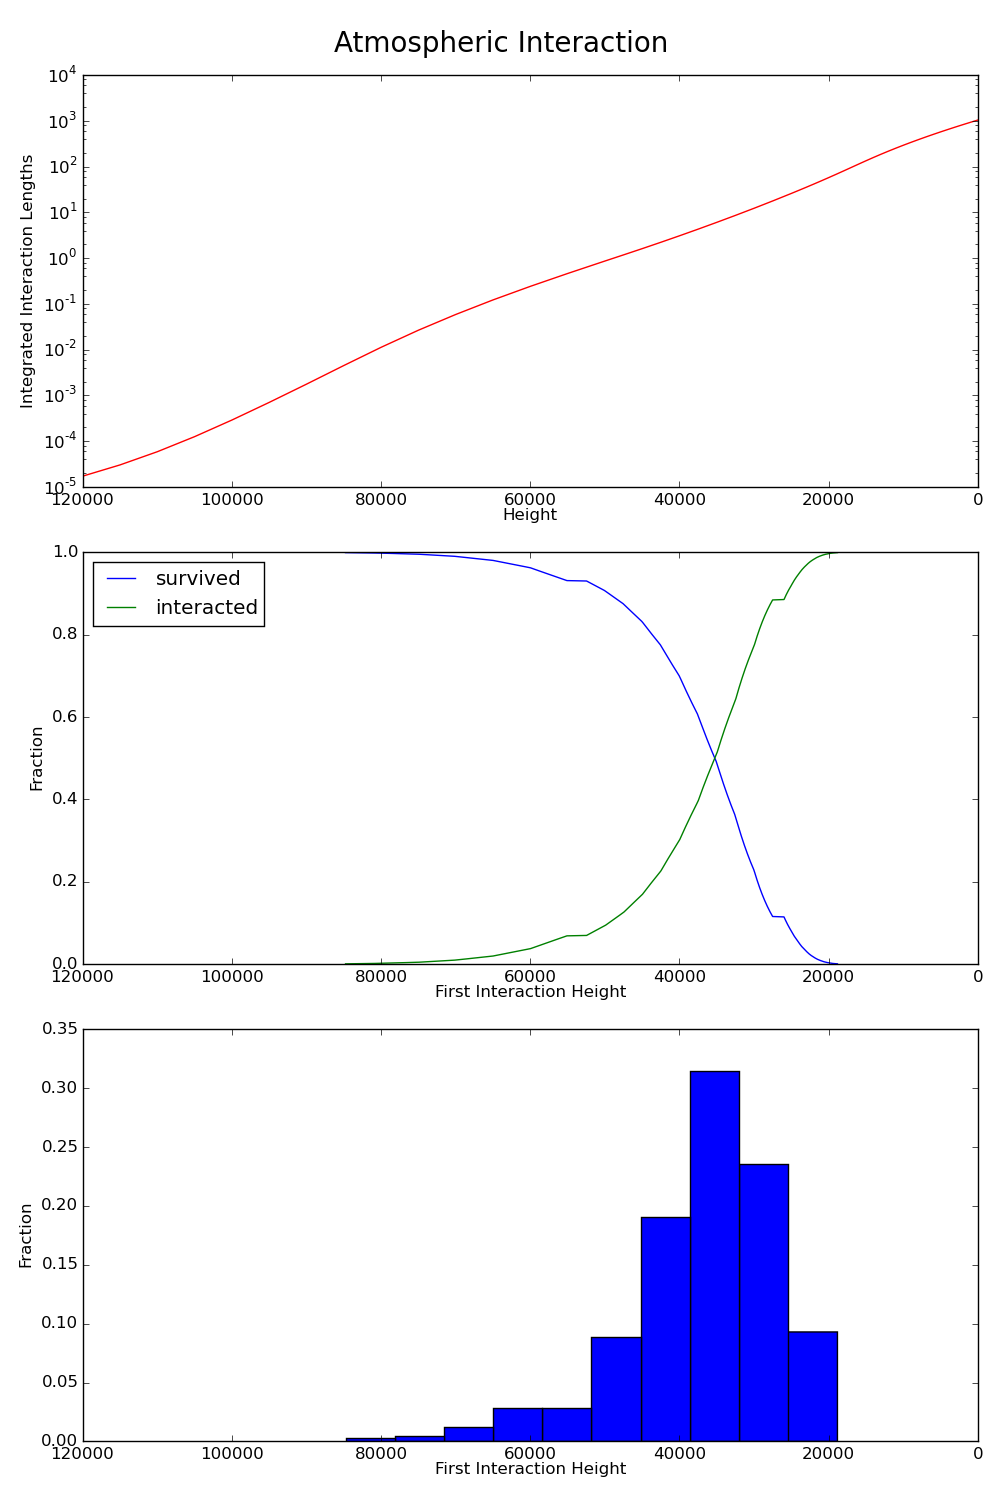
\includegraphics[height=0.9\textheight]{generalheight}
\caption{The integrated interaction lengths increases as height decreases. Thus the decay probability follows a exponentially increasing distribution. The mean first interaction height for all events is roughly 40km above sea level.}
\label{fig:generalheight}
\end{center}
\end{figure}

\subsection{Energy Considerations}
Cosmic Rays follow a well-defined power law where $ \frac{dN(E)}{dt} \propto E^{-\gamma} $ and experimentally $ \gamma = 2.7 \pm ? $. Consequently higher energy Cosmic Rays are heavily suppressed. The Energy Threshold for Cherenkov Light Emission as a function of height is illustrated in \ref{fig:generalenergy}. Once the Energy of a Cosmic Ray exceeds the local Cherenkov Energy Threshold of the atmosphere, the Nucleus will begin emitting a ring of Cherenkov Light. Emission continues until the first interaction with the atmosphere, occurring at a randomly distributed height we call $h$. Then for a given Telescope Array altitude above sea level, simple trigonometry yields the radius of the LDF on the ground:
\[ Radius(height = altitude_{array}) = \tan [\theta_{C}(h)] \times (h - altitude_{array})\]

The Refractive Index of the atmosphere, and thus the Cherenkov angle $\theta_{C}$, increases as the altitude decreases. Thus the upper atmosphere emission contributes to the inner LDF, while the lower atmosphere emission contributes to the outer LDF. We can also see ground emission radius as a function of height in \ref{fig:generalenergy}. We find that the high-radius emission (occurring near the first interaction region) varies little between different high energies. We deem this to be \textquoteleft Saturated Emission\textquoteright.

\begin{figure}
\begin{center}
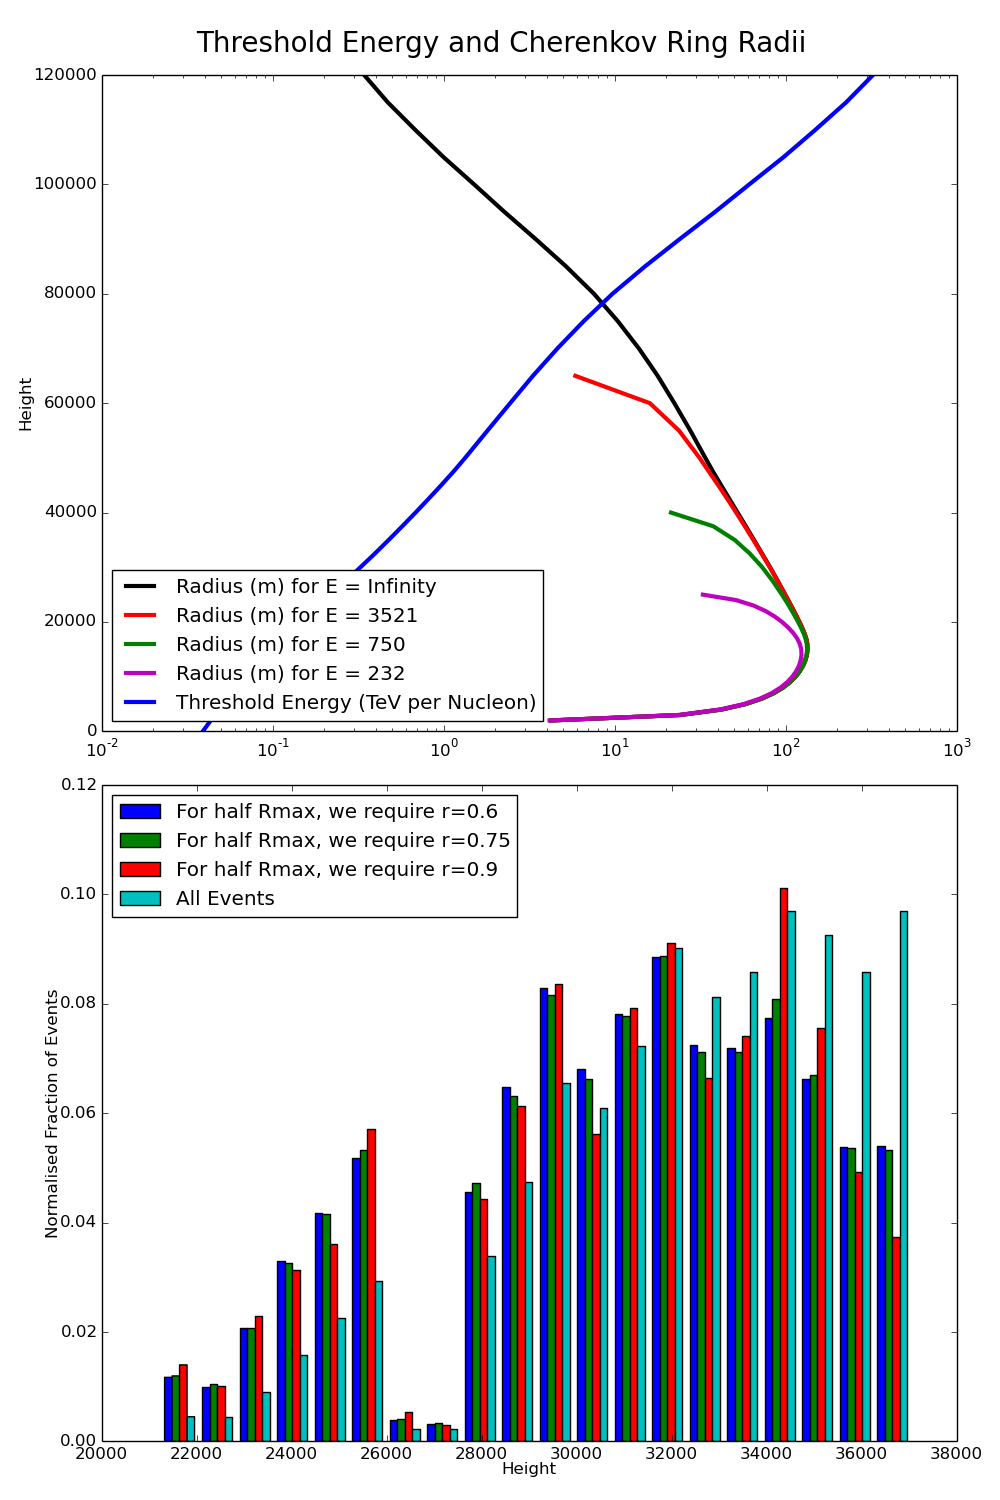
\includegraphics[height=0.9\textheight]{logenergyradius}
\caption{The Threshold Energy for Cherenkov Emission is marked in blue. With the assumption of $\beta=1$, the maximum emission radius is marked in black. The red and green and magenta line show the emission radius at 3.57 and 0.75 and 0.23 TeV per Nucleon respectively. The Green line is sufficiently close to the background to be saturated at 24km, while the magenta line is not.}
\label{fig:generalenergy}
\end{center}
\end{figure}

\subsection{Nuclear Charge}
Cherenkov Emission is determined by the Frank Tamm formula!!!!! 

Under the assumption of constant magnetic permittivity and a zenith angle of $90\degree$ we can use the approximate form \[ N_{photons} \approx (37000 \times Z^{2} \times \Delta_{h} \times \Delta_{E})\] where $\Delta_{h}$ is the vertical distance travelled in meters and $\Delta_{E}$ is the emission energy range in eV.

If we divide the number of emitted photons by the area of the annulus between the ring radii at $h$ and $h - \Delta_{h}$, we retrieve the LDF shown in \ref{fig:lpd}, which varies with $ \rho_{DC}  = f(r) \times Z^{2}$ . Thus the amplitude of the LDF is proportional to the charge of the Cosmic Ray, enabling the Charge to be determined from the DC emission. This is the basis for charge reconstruction in the LDF method.

\begin{figure}
\begin{center}
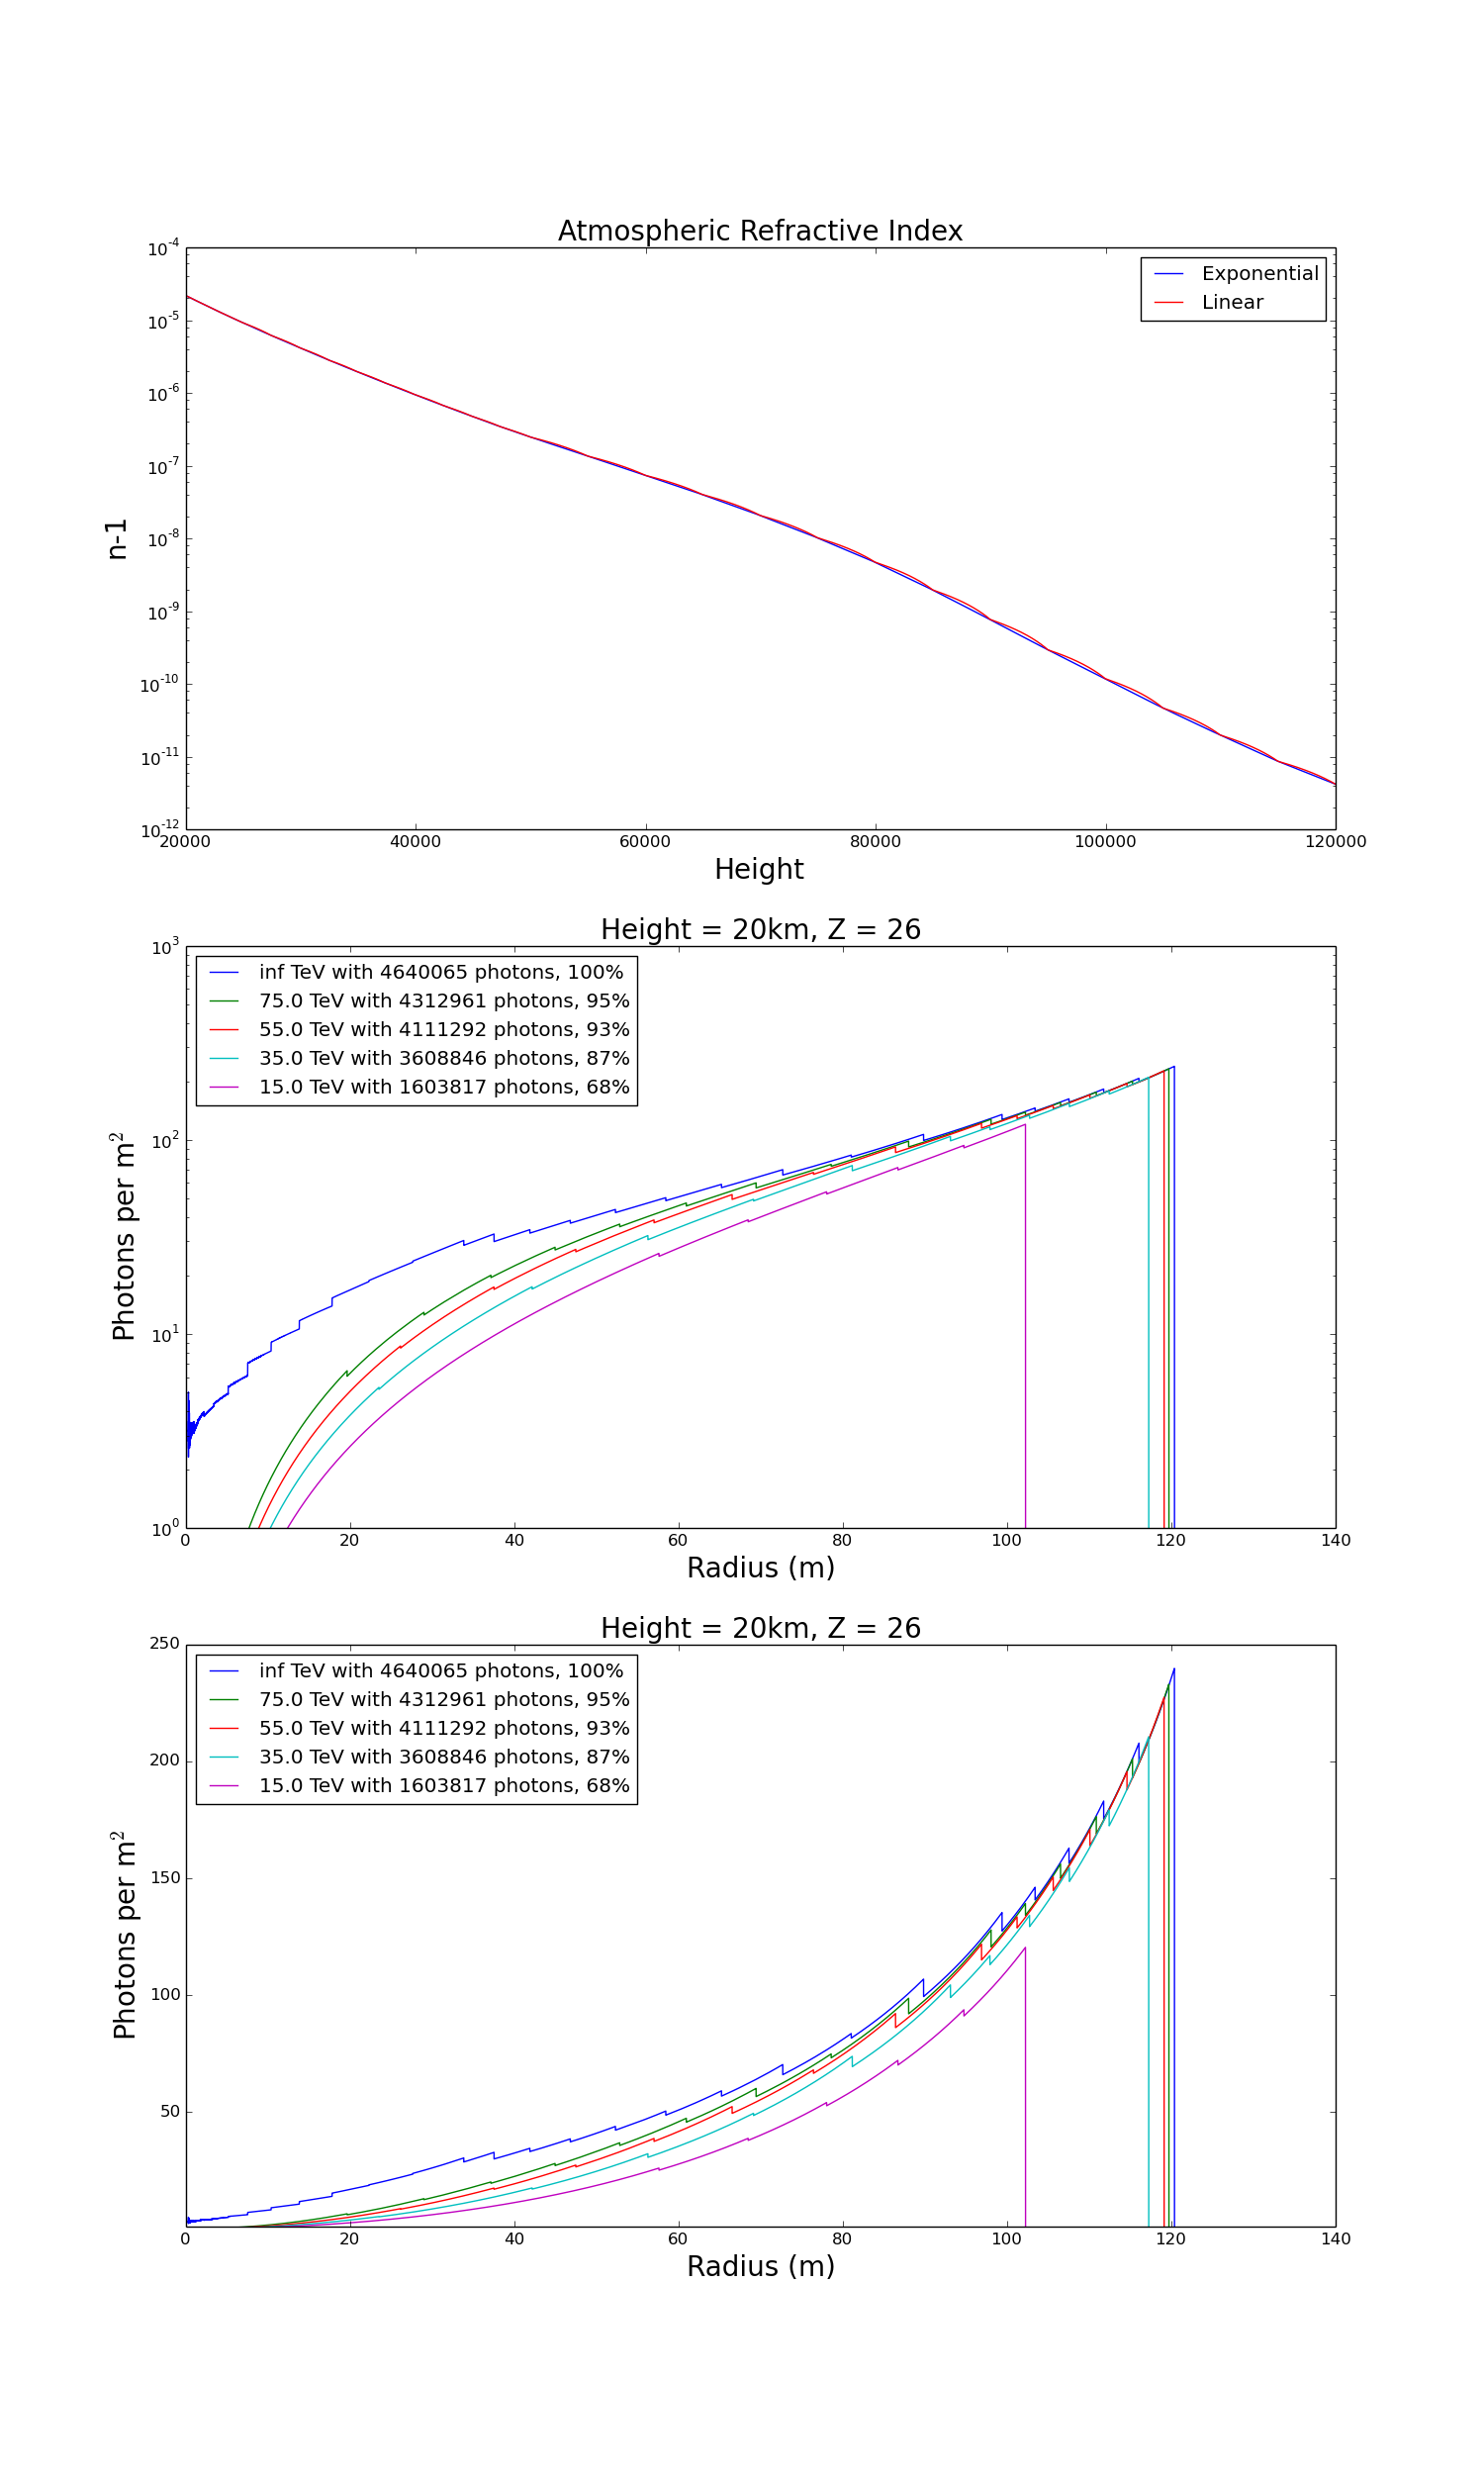
\includegraphics[height=0.9\textheight]{simulatedlpd}
\caption{The LPD obtained from simulation of an Iron Nucleus up to a first interaction height of 25km for a range of Core Energies. An altitude of 1.8km for the experimental array is assumed. Atmospheric absorption, although neglected, is broadly constant across the emission range leading to uniform amplitude scaling.}
\label{fig:lpd}
\end{center}
\end{figure}

\subsection{Energy saturation region}
However, in the 4 telescope height region, the Cherenkov Threshold Energy is $ E_{Threshold} \approx 0.35$ TeV per Nucleon as shown in \ref{fig:lpd}! The saturation in for these heights occurs roughly at 0.7 TeV per Nucleon or something...

\subsection{Atmospheric Absorption}
The Cherenkov Light, mostly emitted in the visible blue part of the EM spectrum, experiences relatively little atmospheric absorption. The major of Rayleigh scattering-based atmospheric absorption occurs in the lower part of the troposphere, and thus the atmospheric absorption is almost independent of emission up to first interaction height.

\section{LPD Event Reconstruction}

\subsection{Log Likelihood Minimisation}
In order to fully reconstruct an event, we need to find the x/y core position, the Energy per Nucleon, the first interaction height and the charge. However, if one telescope in a five-telescope array does not observe DC light, this data point can be used to constrain the core position. Thus, for the LDF method to be applied, we require a minimum of five telescopes, four or more of which must image the DC light. We consider the amount of DC light that each telescope receives to be Poissonian \[  P_{i} ( N_{i, Received} \mid X, Y, Z, height, Epn )  =  \frac{ e^{- \lambda_{i} } \times \lambda_{i} ^{N_{i}} }{N_{i}!} \]

In order to reduce computing time, we can use Stirling's Approximation $\ln( N! )  \approx  N \ln(N) - N + \frac{1}{2} \ln(2 \pi N)$. Pure night sky background requires that there be more that X photons in a DC pixel, and for this Stirling's Approximation has an error of just Y?. We then minimise the Log Likelihood function \[ - \ln(L) = - \sum_{i=1}^{n} \ln(P_{i}) \approx  \sum_{i=1}^{n} [\lambda _{i} - N_{i} \ln(\lambda _{i}) + N_{i} \ln(N_{i}) - N_{i} + \frac{1}{2} \ln(2 \pi N_{i})]  \] where n is the total number of telescopes in the array.

\subsection{Extracting Charge Resolution}
Having reconstructed many events, we can then derive the $\sigma_{Z}$ of the dataset, giving us a number to directly compare the quality of event reconstruction. However, a simple Gaussian 68\% method will yield only half integer values of $\sigma_{Z}$ and very frequently 0. This will be unhelpful for comparisons of minor modifications of reconstruction methods.

Instead, we can assume a Gaussian with tails at the highest and lowest reconstructed charge values in the dataset. The size of the dataset can be used to calculate the fraction of events that the extreme values represent, and this probability can be converted into a \textquoteleft number of standard deviations from mean'. Dividing the Gaussian total width by the number of standard deviations gives us a value for $\sigma$. Although this will in most cases tend to overestimate the spread of the data, it will also be sensitive to all increases in the proportion of correctly reconstructed events.

\subsection{Iterative Scanning Minimisation}
Through $\sigma_{Z}$ calculation, we find that the LDF method initially provides very poor charge reconstruction. This is as a result of varying Threshold Energies and the sharp drop in the LDF above the maximum radius, which means the Log Likelihood is frequently discontinuous within the parameter space. Consequently, a Minuit-type minimisation algorithm will only be able to find a local minimum near the starting values for the fit parameters.

To overcome this problem, we can iterate over a series of starting values for the parameters, with the aim of scanning the true minimum among the many minima found. To simplify matters, we can scan only the integer Z values over the range $ 20 \leq Z \leq 32 $, rather than considering the charge to be a free floating parameter.

In order to reduce the number of calculations needed, we can consider the core position region derived from camera images, as in Hillas Analysis. Each telescope will have a Gaussian smeared central axis indicating the direction of the core. We overlay the simulated telescope array with a grid of points with grid width 1m. Then we select all points satisfy the condition of lying within the shower axis direction confidence interval for every telescope. The angular width of the confidence interval from the shower axis will be determined by the precision of the telescopes.

Having determined the relevant Height and Energy ranges, we can then consider combinations of Energy and Height for which the Energy is above the Cherenkov Emission Threshold (and is saturated!). This gives us a second set of starting \textquoteleft Coordinates \textquoteright.

The Z value is fixed and the LL function is then minimised with the assigned starting values, with the other four variables allowed to float freely. Minimisation typically scans 13 Z values, 10 core position coordinates, and 50 Height/Energy coordinates, yielding $ 13 \times 10 \times 50 = 6500$ minimisations in total. Such a technique is resource intensive but reduces $\sigma_{Z}$ by a factor of 5 or more. (CHECK this quantitatively and get a graph yo. Want to see some plateauing of sigma Z!).

\subsection{Boosted Decision Trees}
Using one quarter of a large sample of Monte Carlo data, we can train a Boosted Decision Tree (BDT) for a given telescope multiplicity, using the reconstructed x/y core position, height and energy, as well as the Log Likelihood. The BDT is told whether each event is \textquoteleft signal' (correctly reconstructed) or \textquoteleft background' (incorrectly reconstructed). 

For every simulated event, this trained BDT can then be used to assign a \textquoteleft Signal Probability'. On a second quarter of the dataset we can optimise a cut on the minimum signal probability, in order to maximise the ratio of signal to background. We find that the $\sigma_{Z}$ of the remaining \textquoteleft Test' Monte Carlo data is reduced when the same BDT cut is applied.

\section{HESS-type Event Reconstruction}
With a simulation of the HESS Cherenkov 5-Telescope Array we can verify the effectiveness of the technique. 
\subsection{First Interaction and Energy Saturation}
The mean first interaction height for all Cherenkov Emitting Cosmic Rays in the atmosphere is 40km, and neglecting variations in atmospheric density profiles around the Earth, this can be considered independent of experimental array. However, the multiplicity of event is determined by equipment efficiencies, altitude and telescope layout. When the HESS layout is simulated, we find that the 4 telescope events have a mean height of $h \approx 23 \pm 5$ km, as shown in \ref{fig:Hessheight}.

\begin{figure}
\begin{center}
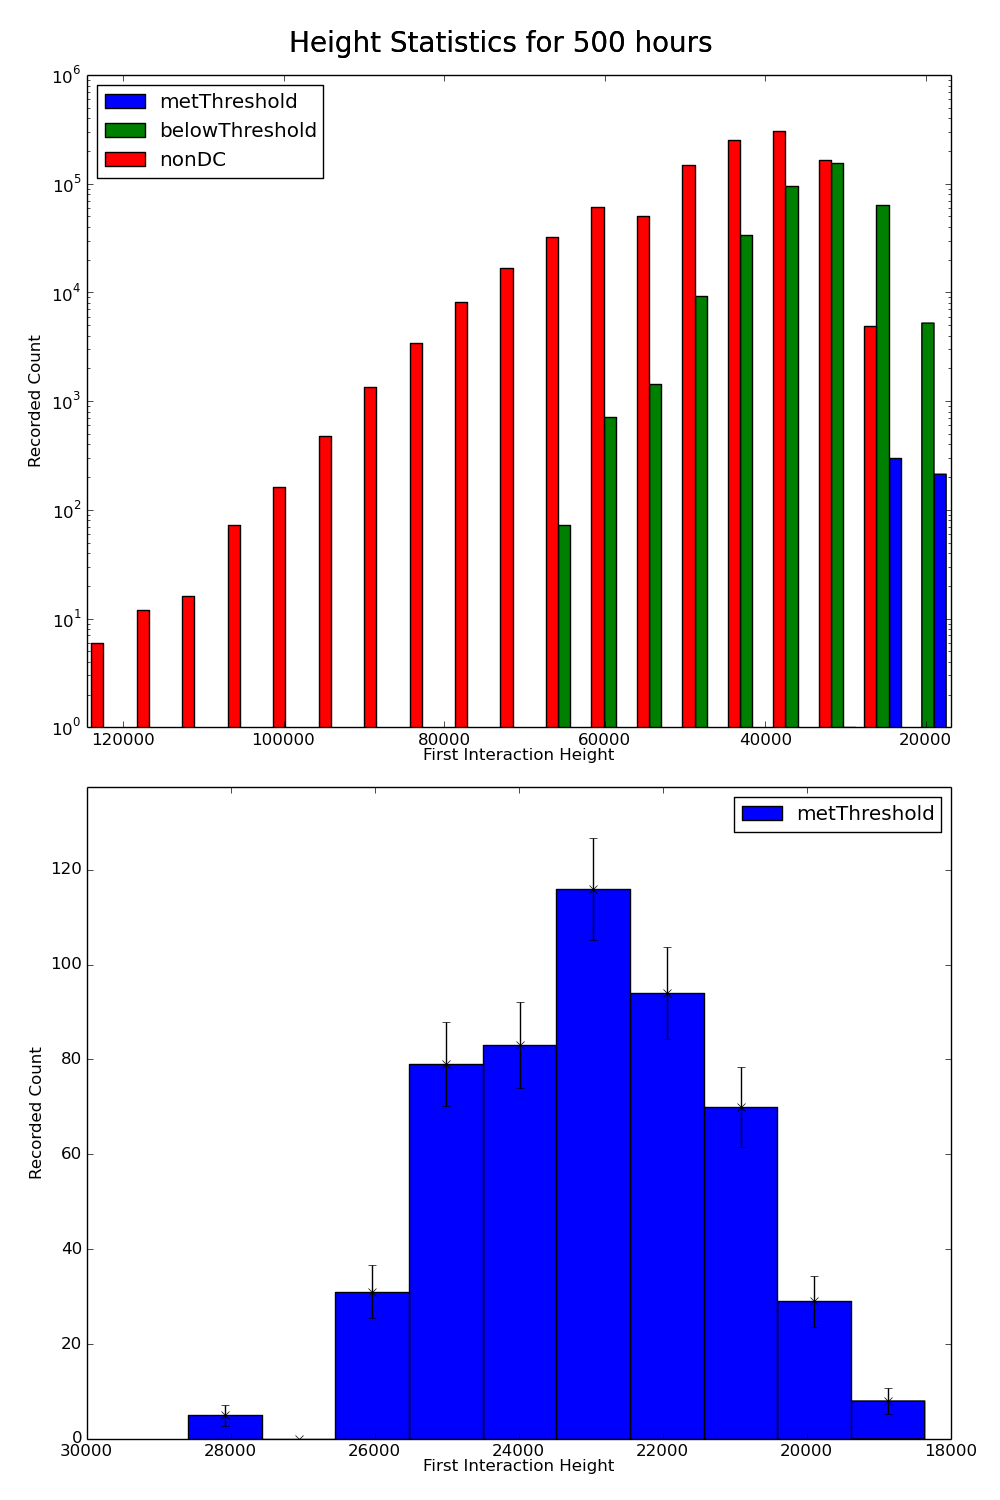
\includegraphics[height=0.9\textheight]{hessheight}
\caption{The mean first interaction height for all Cherenkov Events is 40km???. The mean first interaction height for 4 telescope events in the HESS array is 23km}
\label{fig:Hessheight}
\end{center}
\end{figure}

\subsection{Extended Air Shower Background}
A typical HESS image is shown in \ref{fig:hess}, with the DC pixel visible. For HESS cameras, the Extended Air Shower (EAS) produced after the first interaction of the Cosmic Ray overlaps the DC pixel and thus provides background in the LDF. As the Energy of the Cosmic Ray increases, the EAS speads over a larger angular area, and at smaller radii, the EAS-DC-shower direction axis contracts, leading to more overlap. Thus the background in the DC pixel increases with decreasing radius and increasing Energy. In addition, we have a fixed night sky background with 7 photons $m^{-2}$. We thus parameterise the background with \[ \rho_{bkg}  = 7 + 5E\]. The modeled background LPD is shown as part of REF. It begins to dominate above roughly 1 TeV per Nucleon, particularly in the case of smaller radii. 

\begin{figure}
\begin{center}
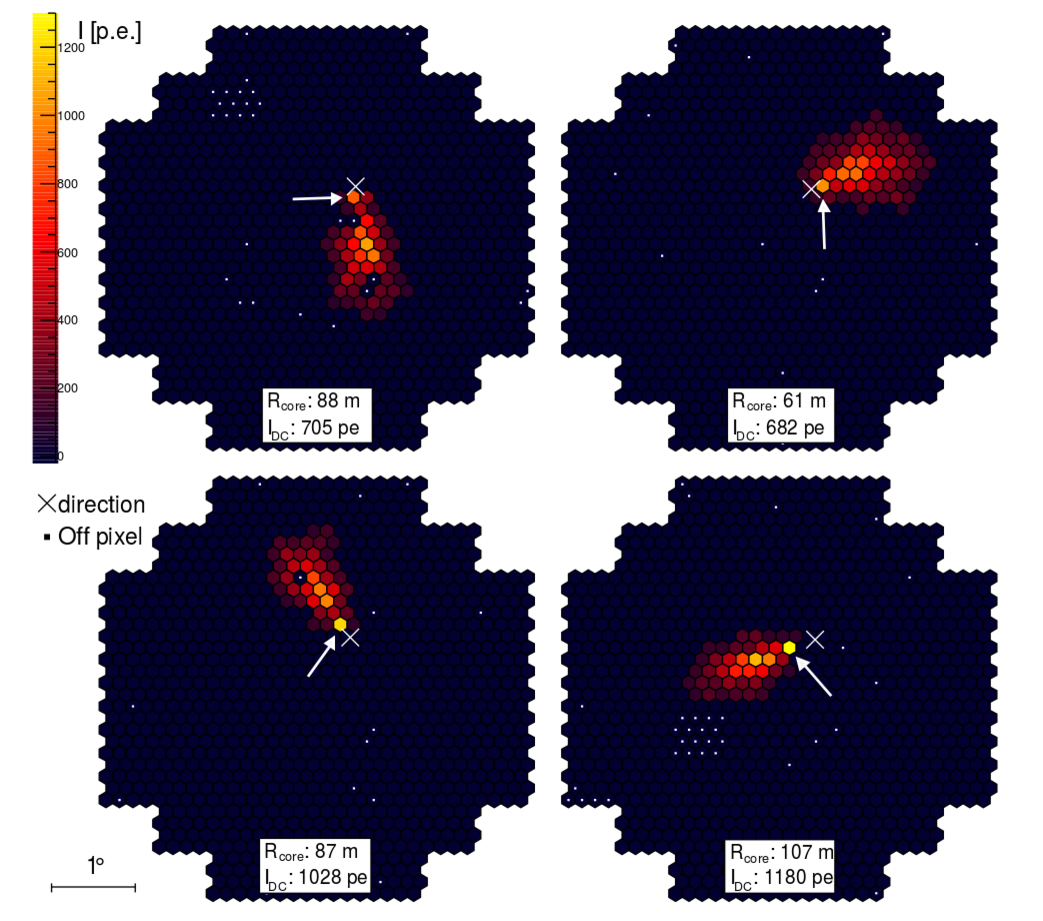
\includegraphics[width=0.9\textwidth]{hess}
\caption{A 4-camera HESS event. The shower direction is marked with a white cross, and the DC pixel is indicated with a white arrow. The shower axis passes through the shower direction, the DC pixel, and the center of the Extensive Air Shower region lying beyond the DC pixel.}
\label{fig:hess}
\end{center}
\end{figure}

\subsection{Reconstructed Charge Resolution}
In the preliminary HESS simulation, it was found that the 4 telescope event reconstruction had a charge resolution of $\sigma_{Z} = 1.4$. However, requiring that the BDT signal probability satisfied $P > 0.81$ removed $75 \%$ of events, while reducing the Charge resolution to $\sigma_{Z} = 0.9$ . With this cut, core position resolution was $d \approx 1.4 m $. For 5 telescope events, it was found that the charge resolution was also $\sigma_{Z} = 1.4$. However, requiring that the signal probability satisfied $P > 0.05$ removed $53 \%$ of events, including all wrongly reconstructed ones. This placed an upper limit on the charge resolution of $\sigma_{Z} < 0.35$ . With this cut, core position resolution was $d \approx 0.8 m $.

However, the simulated number of hours for the data was 1200? hours, and comparisons with HESS data show just 12 4-telescope events rather than 600. Thus, although the technique is valid and effective for HESS, the count rate will limit the potential to conduct any statistical analysis from this experiment.

\section{Optimised Telescope Array}
NO Background!!!!!
\subsection{Count Rates}

In order to improve the count rate of high-multiplicity events, we can consider a 3x3 array of Cherenkov Telescopes, which we want to use for identifying CR Elements accurately. In \ref{fig:optmiselayout} we see that the \textquoteleft High Multiplicity Count Rate' of events observed by 4 or more telescopes falls with increasing grid separation. We can clearly see that the optimum grid spacing will likely lie in the 20-50m region to provide a reasonable count rate. Competing with this effect is the reliance of LDF reconstruction on sampling the entire lateral distribution. Thus the reconstruction quality will decrease as Grid Width decreases. Further study of $\sigma_{Z}$ in this region is required to determine the optimum layout (not necessarily be a grid) for event reconstruction. 

\begin{figure}
\begin{center}
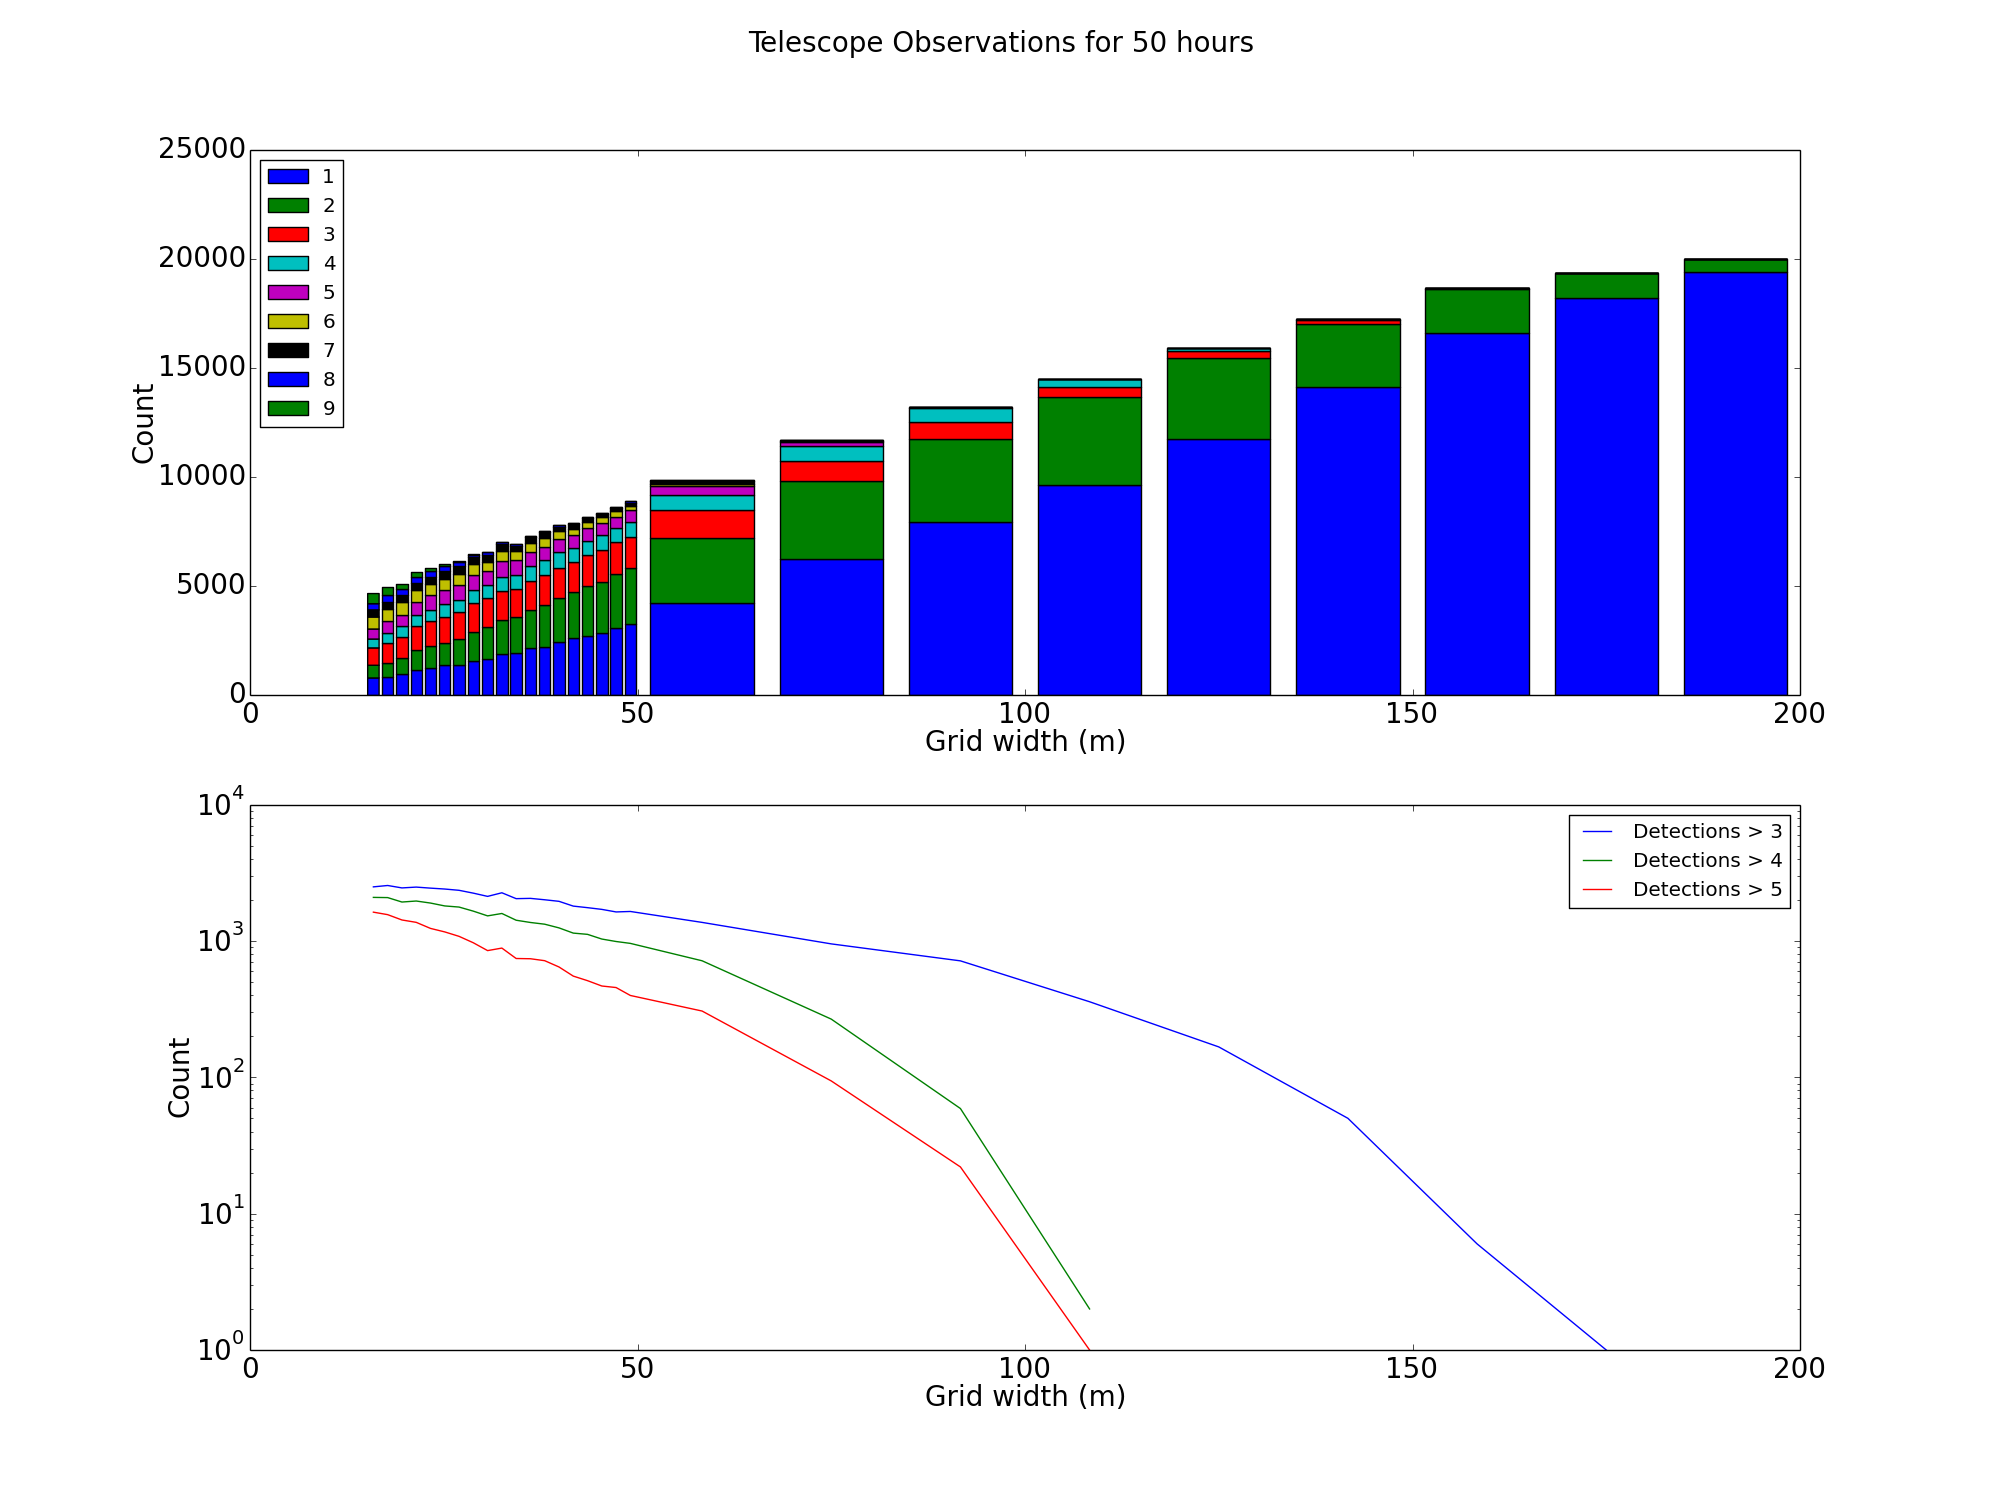
\includegraphics[width=0.9\textwidth]{optimiselayout}
\caption{A simulation of 50 hours of run time for various grid spacing for a 3x3 telescope array. Although raw count rate increases with increasing grid width, the \textquoteleft good count' rate of events observed by sufficient telescopes falls rapidly with increasing grid width}
\label{fig:optmiselayout}
\end{center}
\end{figure}

\subsection{Saturation Region Energies}

\subsection{High Speed Telescopes}
By definition, the EAS shower will arrive on the ground shortly before the DC light. There are currently several high-speed Cherenkov telescopes capable of distinguishing between these, allowing a background-free LDF to be fitted. Additional study of alternative energy regimes and layouts will also be considered for the case of a high-speed imaging telescope array. 

\section{Conclusion}
Preliminary results suggest that the LDF reconstruction technique will significantly improve charge reconstruction, to a level sufficient for cosmic ray abundance studies. However, reliance on high-multiplicity events means that although applicable to current experiments such as HESS, a new optimised telescope array would be required for a statistical analysis. Such an array may have a grid spacing of 20-50m, although further study is needed to determine the ideal layout.
\bibliographystyle{plain}
\bibliography{report}
\end{document}